\subsection{Основные  принципы  построения  и  архитектура  сети  Интернет.  Алгоритмы  и  протоколы  внешней  и внутренней маршрутизации. Явление перегрузки и методы борьбы с ней.}

\textbf{Основные принципы построения сети Интернет}

\begin{enumerate}
    \item \textit{Децентрализация управления} --- нет единого центра управления для сети Интернет.
    \item Выход из строя одного компьютера или участка сети не приводит к неработоспособности всей сети.
    \item \textit{Коммутация пакетов} --- способ динамического распределения ресурсов сети связи за счёт передачи и коммутации оцифрованной информации в виде частей небольшого размера, так называемых \textit{пакетов}, которые передаются по сети, в общем случае, независимо друг от друга (дейтаграммы) либо последовательно друг за другом по виртуальным соединениям. 
    Узел-приёмник из пакетов собирает сообщение. 
    В таких сетях по одной физической линии связи могут обмениваться данными много узлов.
    \item \textit{Инкапсуляция} --- последовательное вложение протокольной единицы (PDU) вышележащего уровня в протокольную единицу нижележащего уровня. 
    PDU вышележащего уровня не доступны на нижележащем уровне (нижележащий уровень не понимает структуры данных вышележащего уровня).
    \item Каждый уровень имеет строго определенный интерфейс с нижележащим и вышележащим уровнями и набор сервисов, которые может использовать вышележащий уровень.
\end{enumerate}

\bigbreak
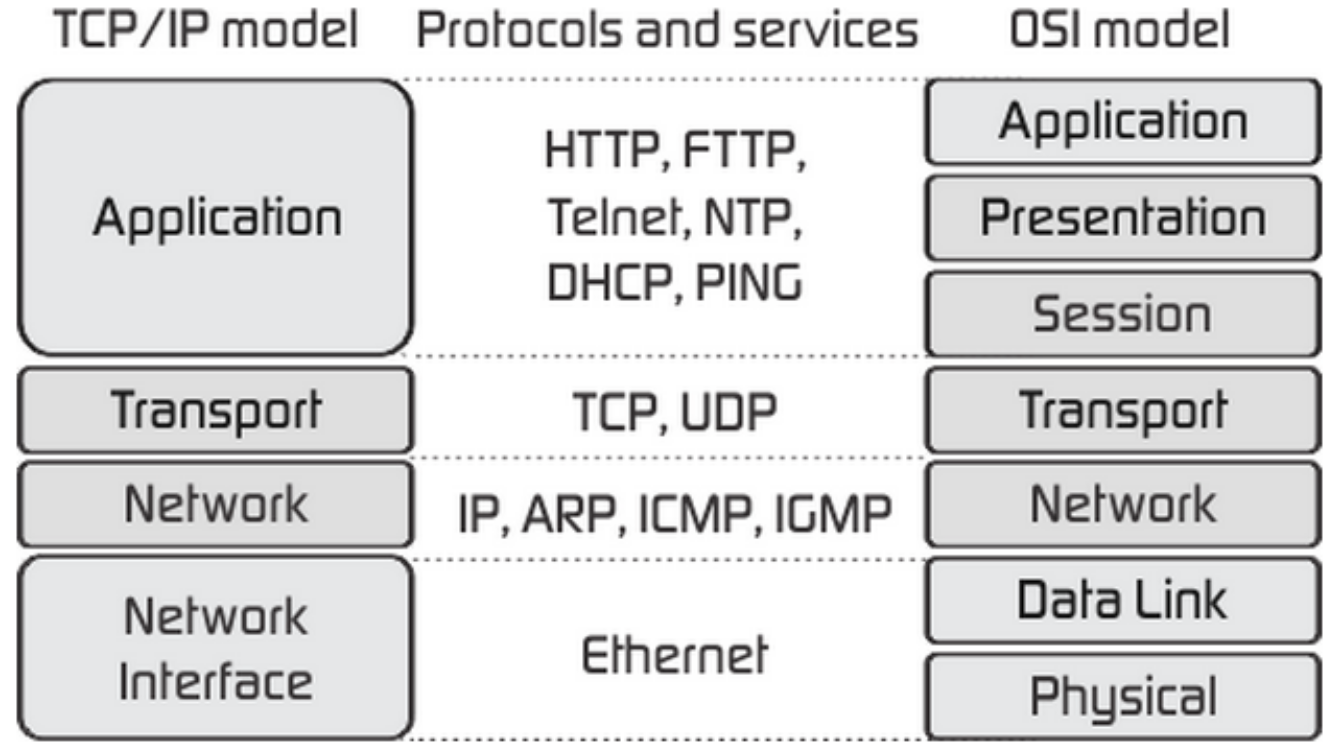
\includegraphics[width=0.2\textwidth]{pics/protocols.png}

\textbf{ISO/OSI:}

\textbf{Физический} -- передача последовательности битов через физическую линию.

\textbf{Канальный} -- превращение несовершенной физической среды передачи данных в надежный канал, свободный от ошибок передачи.

\textbf{Сетевой} -- построение маршрута между отправителем и получателем.

\textbf{Транспортный} -- получение данных с вышерасположенного уровня, разделение на более мелкие единицы (если требуется), передача на сетевой уровень, обеспечение целостности данных при доставке до адресата.

\textbf{Сессии} -- установка сессий между пользователями. Сессия позволяет передавать данные, как это может делать транспортный уровень, и имеет более сложный сервис, полезный в некоторых приложениях. Например, можно осуществить вход в удаленную систему.

\textbf{Представления} -- обеспечение решений проблем, связанных с представлением данных, в основном — проблемы синтаксиса и семантики передаваемой информации.

\textbf{Приложений} -- обеспечение работы часто используемых приложений, например — передача файлов.


%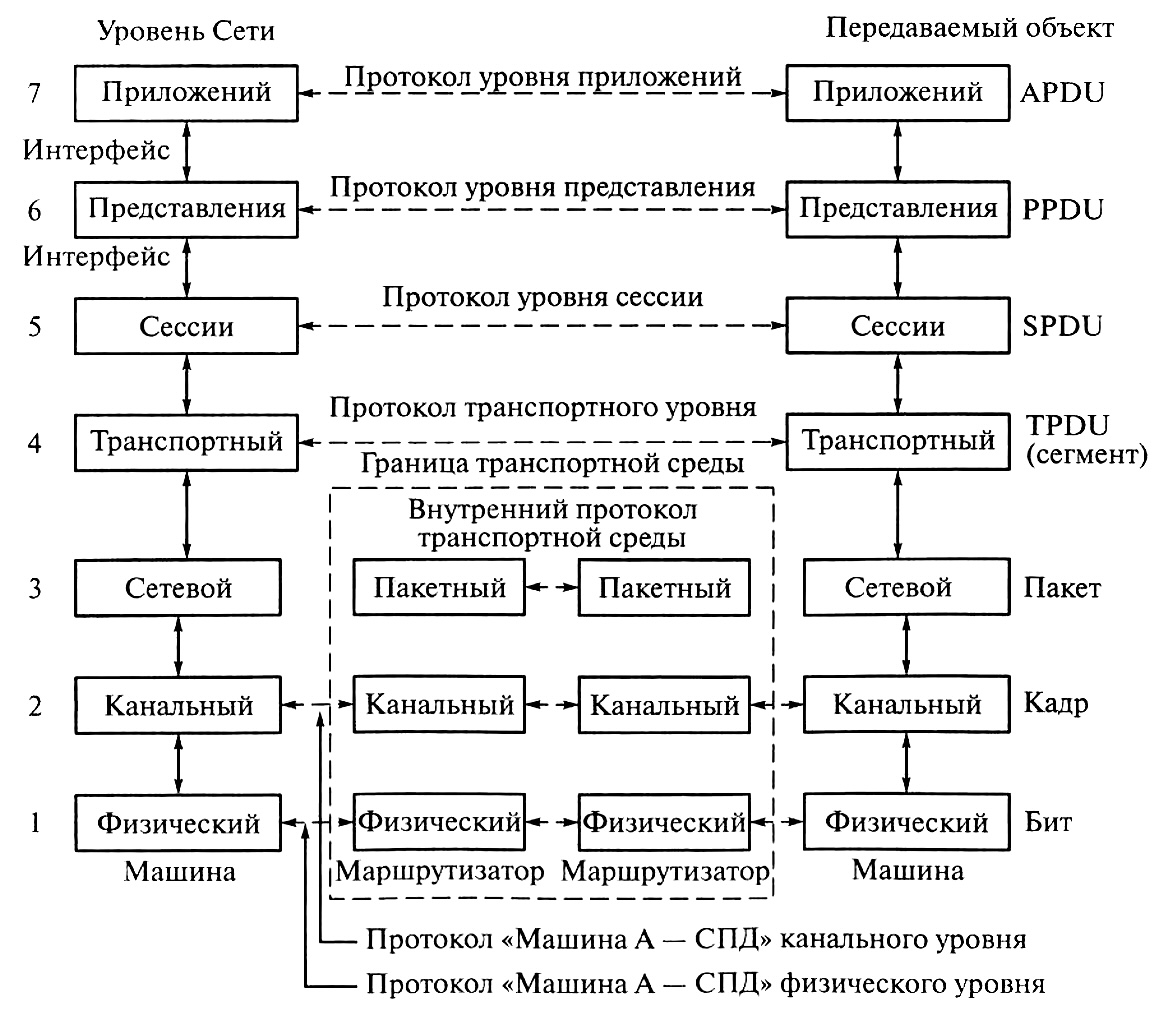
\includegraphics[width=0.24\textwidth]{pics/iso_osi.jpg}
%(PDU -- Protocol Data Unit)

\bigbreak
\textbf{TCP/IP:}

\textbf{Прикладной уровень}.
На прикладном уровне (Application layer) работает большинство сетевых приложений.
Эти программы имеют свои собственные протоколы обмена информацией, например, интернет браузер для протокола HTTP, ftp-клиент для протокола FTP (передача файлов).

\textbf{Транспортный уровень} (как упаковывать?).
Протоколы транспортного уровня (Transport layer) могут решать проблему негарантированной доставки сообщений («дошло ли сообщение до адресата?»), а также гарантировать правильную последовательность прихода данных.

\textbf{Сетевой (межсетевой) уровень} (кому отправлять?).
Межсетевой уровень (Network layer) изначально разработан для передачи данных из одной сети в другую. На этом уровне работают маршрутизаторы, которые перенаправляют пакеты в нужную сеть путём расчёта адреса сети по маске сети.

\textbf{Канальный уровень} (как кодировать в среде?).
Канальный уровень (англ. Link layer) описывает способ кодирования данных для передачи пакета данных на физическом уровне (то есть специальные последовательности бит, определяющих начало и конец пакета данных, а также обеспечивающие помехоустойчивость).

% Снизу вверх: машина СПД (сети передачи данных), межсетевой уровень, транспортный уровень, уровень приложений.

% Модель никак не регламентирует организацию и функционирование сети передачи данных, ровно как и связь с ней, поэтому про уровень машины СПД сказать нечего.

% В модели нет уровня сессий и уровня представлений, поскольку необходимость в них была неочевидна для ее создателей. 

% Остальные уровни соответствуют одноименным уровням модели ISO/OSI.

\bigbreak
\textbf{Алгоритмы и протоколы внешней и внутренней маршрутизации}

Алгоритмы маршрутизации применяются для определения наилучшего пути пакетов от источника к приёмнику и являются основой протокола маршрутизации. 
Для формулирования алгоритмов маршрутизации сеть рассматривается как граф. 
При этом маршрутизаторы являются узлами, а физические линии между маршрутизаторами --- рёбрами соответствующего графа.
Каждой грани графа присваивается определённое число --- стоимость, зависящая от физической длины линии, скорости передачи данных по линии или стоимости линии.
Основными алгоритмами являются алгоритмы Беллмана-Форда и Дейкстры.

\textbf{Алгоритм Беллмана-Форда} (пример алгоритма по вектору расстояний):

\begin{itemize}
    \item Пусть каждый маршрутизатор знает стоимость линии к каждому своему непосредственному соседу
    \item Маршрутизатор $R_8$ рассчитывает стоимость $C_i$ для достижения каждого известного ему $R_i$
    \item Вектор $C_8 = (C_1,C_2,...,C_7)$ - вектор расстояния до $R_8$
    \item Изначально $C = (\infty,\infty,...,\infty)$
    \begin{enumerate}
        \item Каждые $T$ секунд $R_i$ шлёт $C_i$ всем свои соседям
        \item Если $R_i$ нашёл более дешёвый путь, то он обновляет $C_i$ у всех своих соседей
        \item Вернуться к 1
    \end{enumerate}
    \item Длину вектора $C$ устанавливает администратор
\end{itemize}

\textbf{Алгоритм Дейкстры} (пример алгоритма по состоянию канала):

\begin{enumerate}
    \item Определение топологии сети: каждый маршрутизатор передаёт лавиной всем своим соседям состояния своих линий и строит топлогию сети (1. Периодически, 2 Когда изменяется состояние линии)
    \item Вычисление по алгоритму Дейкстры: каждый маршрутизатор независимо запускает алгоритм Дейкстры наикратчайшего пути.
    Каждый маршрутизатор находит соединяющее дерево с минимальной стоимостью до каждого другого маршрутизатора.
\end{enumerate}

\textit{Протоколы внутренней маршрутизации}: RIP (на основе алгоритма Б-Ф, редко используется), OSPF (на основе алгоритма Д, широко используется).

\textit{Протоколы внешней маршрутизации}: BGP-4 --- алгоритм разработан для того, чтобы решить проблему того, что Интернет представляет из себя смесь разнообразных автономных сетей. Необходимо учитывать ряд условий, связанных с политикой автономной сети, например, пакеты из Министерства обороны не должны проходить через недружественные страны.


\textbf{Перегрузка} --- падение производительности в транспортной среде из-за слишком большого числа пакетов. (Если на маршрутизаторе в очереди скапливается много пакетов, то они просто сбрасываются -- это неэффективно)

\textbf{Управление перегрузками} --- организация потоков в транспортной среде, при которой потоки соответствуют пропускной способности подсети и не превышают ее.
% \begin{itemize}
%     \item \textit{Перегрузка} --- падение производительности в транспортной среде из-за слишком большого числа пакетов. (Если на маршрутизаторе в очереди скапливается много пакетов, то они просто сбрасываются -- это неэффективно)
%     \item \textit{Управление перегрузками} --- организация потоков в транспортной среде, при которой потоки соответствуют пропускной способности подсети и не превышают ее.
%     \item \textit{Методы, предотвращающие перегрузки:}
%     \begin{enumerate}
%         \item Схема управления потоком (небольшое окно) сдерживает нарастание трафика и предотвращает появление перегрузок.
%         \item Методы управления очередями, организация очередей: одна общая на входе или одна общая на выходе; по одной на каждую входную линию или на каждую выходную; по одной очереди на каждую входную и выходную --- все это влияет на появление перегрузок.
%         \item Выбор метода сброса пакетов также влияет на перегрузки. 
%         Правильная маршрутизация, равномерно использующая каналы в транспортной среде, позволяет избежать перегрузки.
%         \item Методы, регулирующие время жизни пакета в сети, также влияют на образование перегрузок.
%     \end{enumerate}
% \end{itemize}


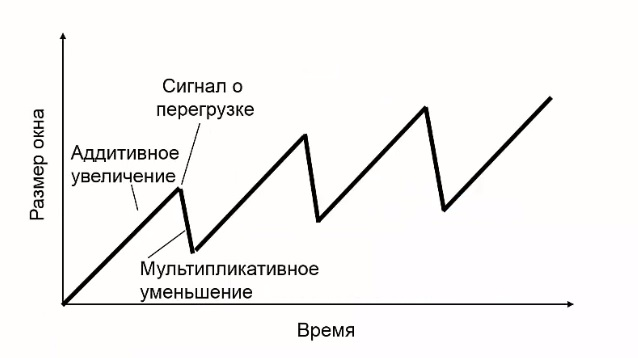
\includegraphics[width=0.75\columnwidth]{pics/dop16_add.jpg}

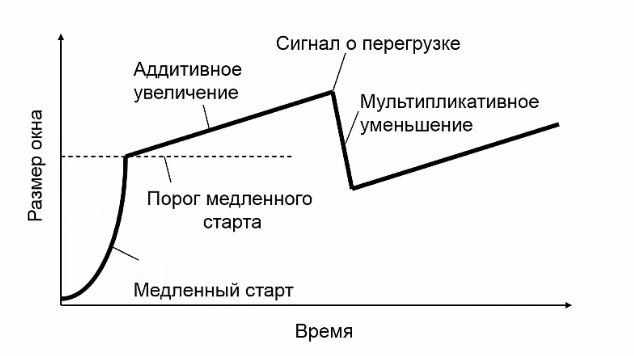
\includegraphics[width=0.75\columnwidth]{pics/dop16_mul.jpg}

% -------- source --------
\bigbreak
[\cite{smelbook1}]
[\cite{smelbook2}]